%%%%%%%%%%%%%%%%%%%%%%%%%%%%%%%%%%%%%%%%%%%%%%%%%%%%%%%%%%%%%%%%%%%%%%%%%%%%%%%%%%%%%%%%%%%%%%%%%%%
% Chapter 5 -> Methods for TI
% Author: Mingbo Cheng
%%%%%%%%%%%%%%%%%%%%%%%%%%%%%%%%%%%%%%%%%%%%%%%%%%%%%%%%%%%%%%%%%%%%%%%%%%%%%%%%%%%%%%%%%%%%%%%%%%%
%\addbibresource{~/MEGA/MEGAsync/phd/thesis_Cheng/preamble/thesis.bib}
\chapter{Methods for Trajectory Inference}
\label{chapter:methods_TI}
\graphicspath{{chapter5/figs}}

In the previous two chapters, we presented the implementation of single-cell integration methods and the benchmarking to validate our MOJITOO method. With a shared latent space, we can further perform several downstream analyses, among which trajectory inference is crucial for capturing cell differentiation. Inferring trajectories is challenging since we can only capture specific time points of single cells rather than the dynamic process. Trajectory inference for single-cell multimodal data provides an opportunity to delve deeper into biological processes.

This chapter exclusively introduces the formalization and implementation of our novel trajectory inference method for single-cell multimodal data. We first introduce the necessary notation for the method (\sref{TI_methods:notation}). Next, we present the implementation details of trajectory inference, specifically focusing on graph triangulation, Hodge decomposition, and tree creation (\sref{TI_methods:TI}). Following that, we describe the implementation details of our package (\sref{TI_methods:implementation}). Finally, we conclude this chapter by discussing the strengths of our method (\sref{TI_methods:discussion}).


\section{Notation} \label{TI_methods:notation}
$\mathcal{V}: $ A set of vertices\\
$\mathcal{S}^k = \{{v}_0,\cdots,{v}_k \}: $ A $k$-simplex\\
$\mathcal{X}: $ A simplicial complex.\\
$\mathcal{C}_k(\mathcal{X}): $ Vector space with coefficients in $\mathbb{R}$ whose basis is the set of oriented k-simplices of $\mathcal{X}$\\
$\partial_k ([v_0,\cdots, v_k])$: boundary map\\
$\mathbf{B}_k: $ A k order incidence matrix.\\

\section{Trajectory Inference}
\label{TI_methods:TI}

\subsection{Simplicial Complex}



A $k$-simplex~\citep{schaub2021signal}~(\fref{fig:simplex}) $\mathcal{S}^k = \{{v}_0,\cdots,{v}_k \}$ is an unordered subset of a finite set of vertices $\mathcal{V}$ with cardinality $k + 1$, where $v_i\in \mathcal{V}$, $v_i \neq v_j$ and $i \neq j$.

\begin{figure}[!h]
    \centering
    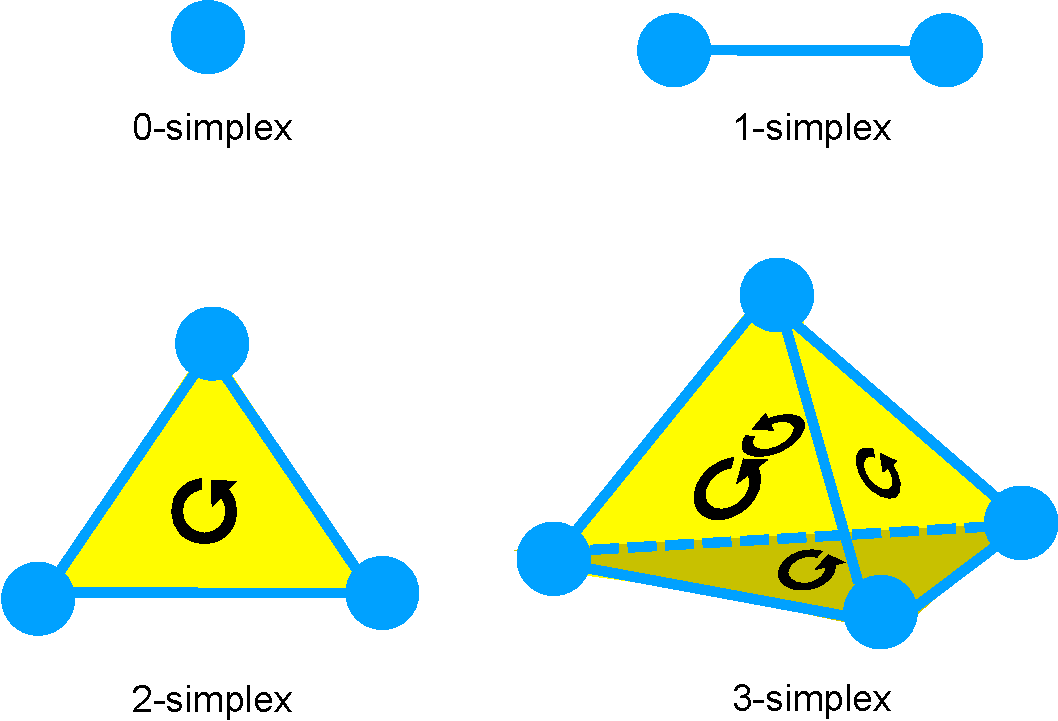
\includegraphics[width=0.45\textwidth]{Simplex/fig}
    \vspace{0.1cm}
    \caption[0-simplex to 3-simplex.]{0-simplex to 3-simplex.}
    \label{fig:simplex}
\end{figure}

A simplicial complex~(SC)~(\fref{fig:sc}) $\mathcal{X}$ is a collection of simplices, where for all $k$-simplices $\mathcal{S}^k$ in $\mathcal{X}$, any subset of $\mathcal{S}^k$ must also be in $\mathcal{X}$. The typical $0$-simplices, $1$-simplices, $2$-simplices are also respectively called vertices, edges and triadic faces. A face of a simplex $\mathcal{S}^k$ is a subset of $\mathcal{S}^k$  with cardinally $k$ in the form $\{v_0 \cdots v_{i-1}, v_{i+1}\cdots v_k\}$ for $0 \leq i \leq k$. A co-face $\mathcal{S}^{k+1}$ of a simplex $\mathcal{S}^k$ is a $(k + 1)$-simplex such that $\mathcal{S}^k$ is a subset of $\mathcal{S}^{k+1}$.  When ordering vertices of a $k$-simplex $\{{v}_0,\cdots,{v}_k \}$, it becomes an orientated $k$-simplex denoted by $[{v}_0,\cdots,{v}_k ]$, where the orientation changing corresponds to the change of sign of the coefficient, i.e. $[{v}_0,\cdots {v}_i, \cdots {v}_j\cdots,{v}_k ]$ = $-[{v}_0,\cdots {v}_j, \cdots {v}_i\cdots,{v}_k ]$.

\begin{figure}[!h]
    \centering
    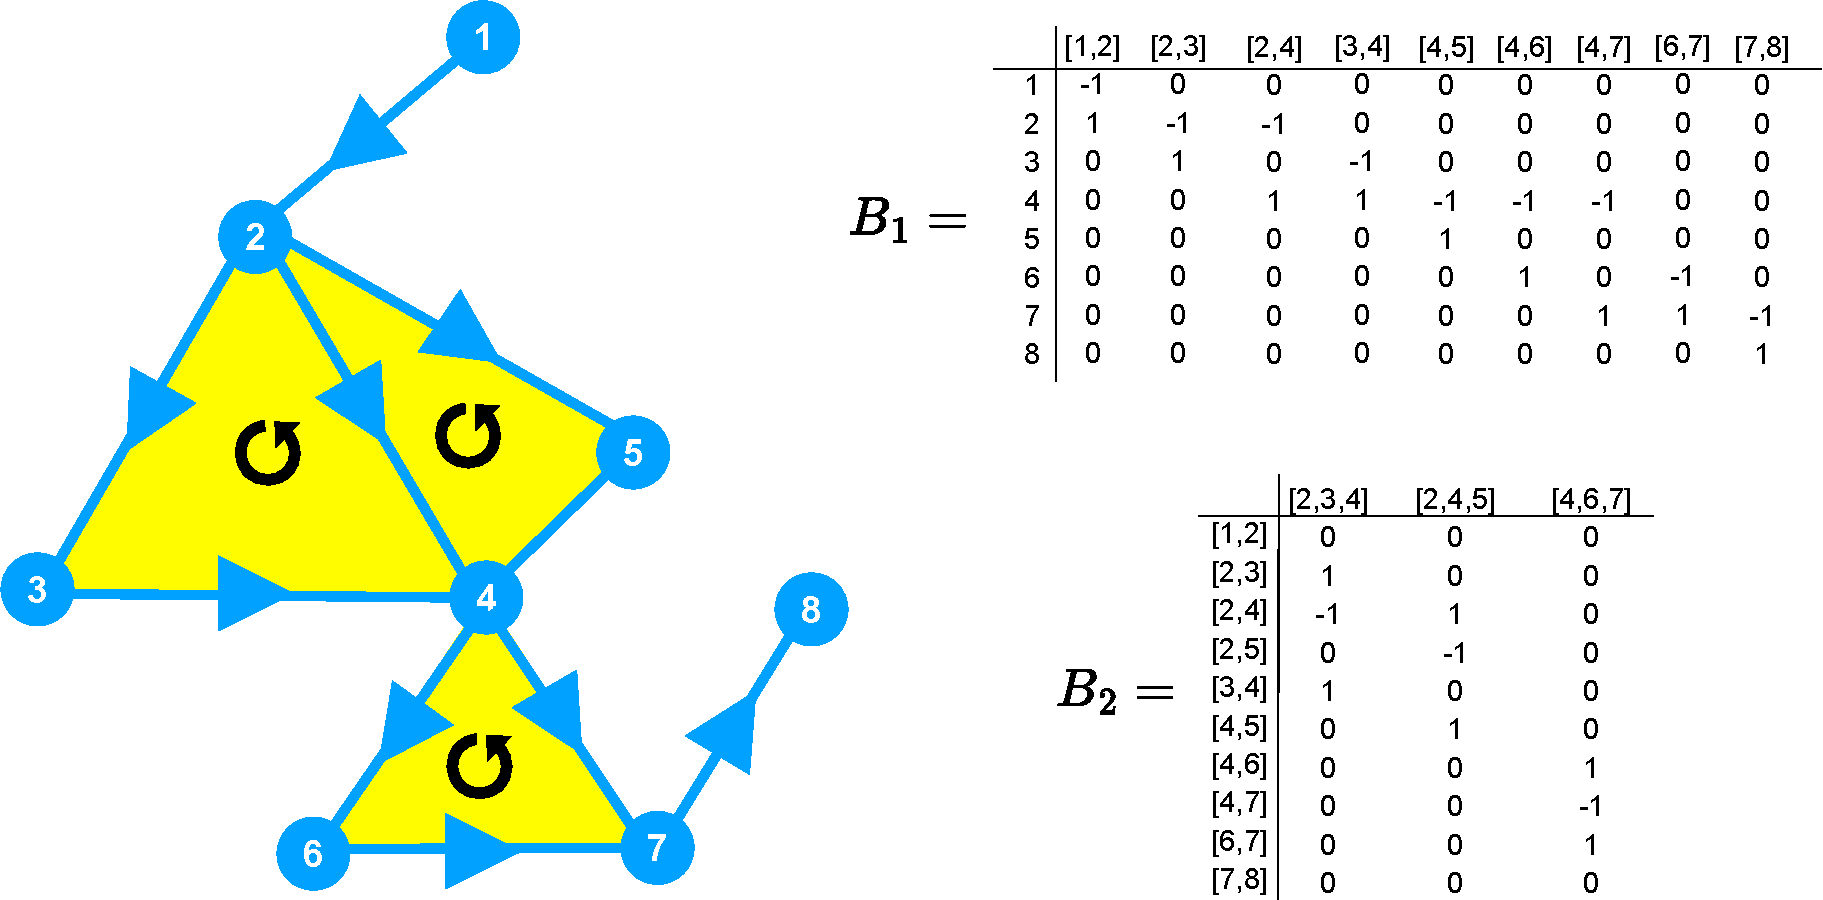
\includegraphics[width=0.65\textwidth]{Simplicial_Complex/fig}
    \vspace{0.1cm}
    \caption[A simplicial complex example.]{Example of a ordered simplicial complex and boundary maps $\mathbf{B}_1$ and $\mathbf{B}_2$ representing this
complex.}
    \label{fig:sc}
\end{figure}


For each $k \geq 0$, $\mathcal{C}_k(\mathcal{X})$ is the vector space with coefficients in $\mathbb{R}$ whose basis is the set of oriented k-simplices of $\mathcal{X}$. $\mathcal{C}_k(\mathcal{X}) = 0$ when $k$ is larger than the dimension of $\mathcal{X}$. An element of these vector spaces $c_k \in \mathcal{C}_k(\mathcal{X})$ is called a $k$-chain, which is a linear combination of the basis elements. The boundary map is defined as the linear transformations $\partial_{k}$: $\mathcal{C}_k(\mathcal{X}) \rightarrow \mathcal{C}_{k-1}(\mathcal{X})$ acts on basis elements as follows:
\begin{equation}
\partial_k ([v_0,\cdots, v_k]) = \sum_{i=0}^{k} (-1)^i [v_0, \cdots, v_{i-1}, v_{i+1}, \cdots, v_k]
\end{equation}
$\mathrm{im}(\partial_k)$ is the space of $(k-1)$-boundaries, where $\mathrm{im}(.)$ is the image of an operator. We can construct the matrix representation of the boundary operators $\partial_k$ by $\mathbf{B}_k$~\citep{lim2020hodge,muhammad2006control}. For example, as shown in~\fref{fig:sc}, the incidence matrices $\mathbf{B}_1$ and $\mathbf{B}_2$ of the 2-simplicial complex capture the relationships between nodes and edges, and edges and triangles, respectively.

\begin{figure}[!ht]
	\centering
	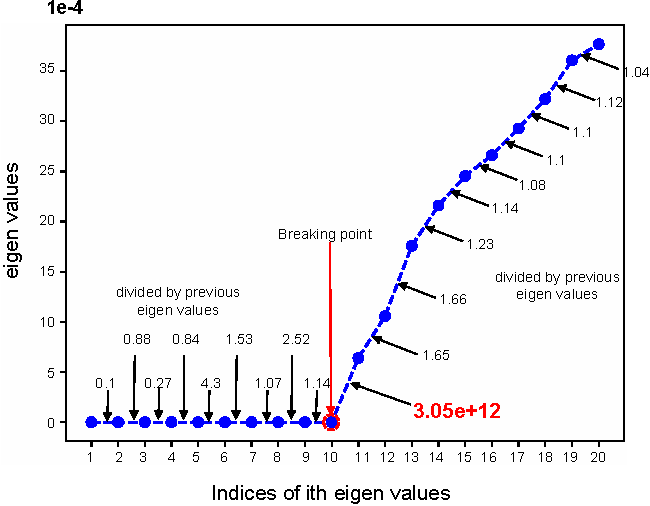
\includegraphics[width=0.65\textwidth]{breakingpoint/fig}
	\vspace{0.1cm}
	\caption[Number of eigens selecting algorithm.]{\textbf{Number of eigens selecting algorithm.} The eigenvalues are derived from the benchmarking data, specifically from the Diffusion Limited Aggregation Tree with 10 branches.}
	\label{fig:breakingpoint}
\end{figure}


\begin{figure}[!ht]
    \centering
    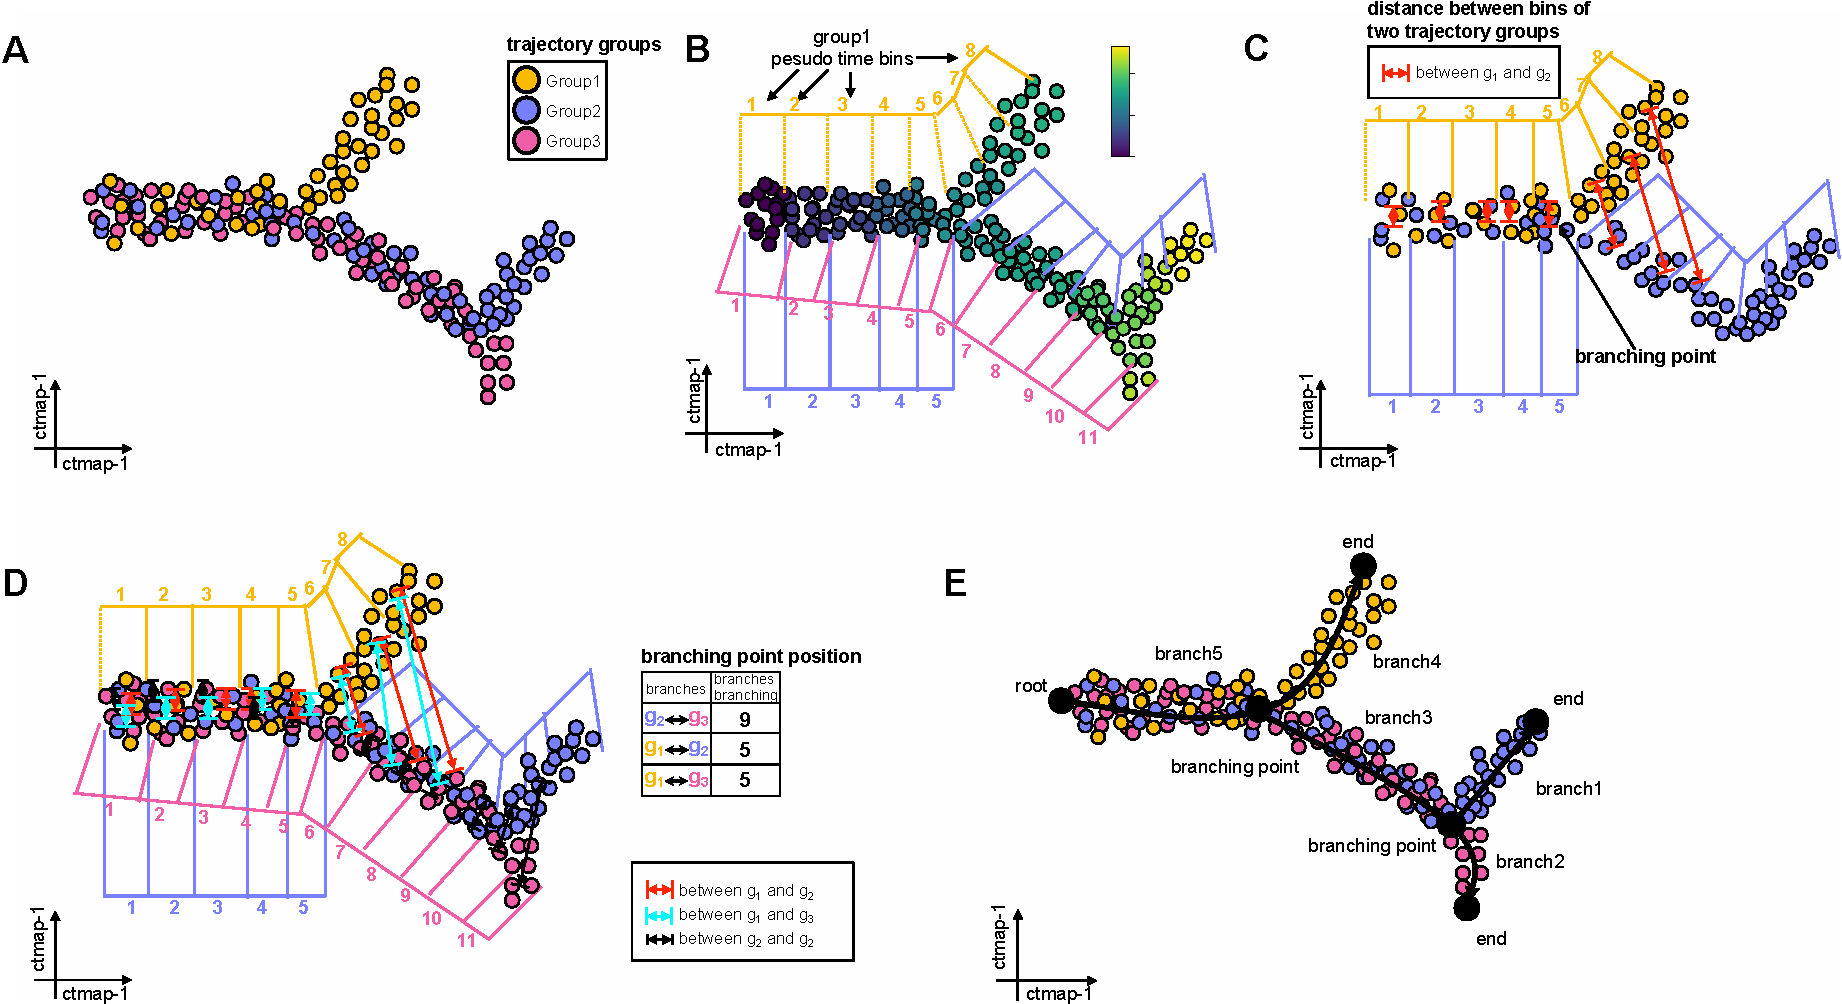
\includegraphics[width=0.65\textwidth]{branching/fig}
    \vspace{0.1cm}
    \caption[Schematic showing how to create a PHLOWER tree.]{\textbf{Schematic showing how to create a tree using edges lay in cumulative trajectory space.}  \textbf{A)}Example of three trajectory groups g1 , g2 , g3 each with a distinct color in the cumulative trajectory space. Every dot in this embedding represents a edge in the graph (or a cell differentiation event). \textbf{B)} PHLOWER takes the mean on the pseudo-time of the vertices (cells) connected by an edge and use this an the edge pseudo-time estimate. PHLOWER next bins the edges by considering their pseudo-times. \textbf{C)} It then estimate average edge locations for every bin, which serves as a backbone for the trajectories. It also estimate distance between edges in two groups but with the same bin index. \textbf{D)} Distance between bins are estimated for all groups and branchings points are detected whenever distance between edges in two groups surpasses the distances of edges within a group for a given bin In the example, bin 9 is a branching point between groups 2 and 3 and bin 5 is a branching point between groups 1 and 2 and 1 and 3. \textbf{E)} To build the final tree, PHLOWER considers the branching points with the highest values towards the lowest values to build trees in a bottom-up approach, i.e. it merges trajectory 2 and 3 at bin 9. The next branching point is 5, which connects trajectory 1 with the tree formed by 2 and 3.}
    \label{fig:branching}
\end{figure}



\begin{algorithm}
    \Input{
        $A$, Affinity matrix\\
        $W$, Diffusion distance matrix\\
        $G^{t}=\{\mathcal{V}^{t},\mathcal{E}^{t}\}$, Triangulated graph\\
    }
    \Parameter{
        $N$, Number of trajectories\\
        $K=9$, KNN graph using A, W\\
        $\text{pct}$, Percentage of starting cells\\
    }
    \Output{
        $L_p$, The list of trajectories\\
    }

    $i \gets 1$ \\
    $G^{knn}=\{\mathcal{V}^{knn}, \mathcal{E}^{knn}\} \gets \textbf{Graph}(A,W,K)$ \\
    $\mathcal{V}_{low}^{knn} \gets \textbf{LowestPseudotime}(\mathcal{V}^{t}, \text{pct})$ \Comment*[r]{pct is percentage parameter}
    $U[v] \gets \textbf{PesudoTime}(v)$ \Comment*[r]{Pseudo time of node v}
    $L_p \gets [()_{1}, ()_{2}, \cdots ()_{N}]$\\
    \While{$i \leq N$}
    {
        $l_{temp} \gets ()$ \\
        $\text{node} \gets \textbf{random}(\mathcal{V}_{low}^{knn})$ \\
        $l_{temp} \gets \textbf{Append}(l_{temp}, \text{node})$ \\
        \While{$\textup{\textbf{true}}$}{
            $\text{NextNodes} \gets \{\mathcal{V} | \mathcal{V}\in \textbf{Neighbor}(\mathcal{E}^{knn}, \text{node}) \text{ and } U[\mathcal{V}]>U[\text{node}]  \}$\\
            \If{$\textup{NextNodes} == \emptyset$}{
                \textbf{break}
            }
            $\text{NextNode} \gets \textbf{PropRandom}(\text{NextNodes})$ \\
            $l_{temp} \gets \textbf{Append}(l_{temp}, \text{NextNode})$ \\
            $\text{node} \gets \text{NextNode}$\\
        }
        $\text{Len} \gets \textbf{Length}(l_{temp})$\\
        $k \gets 1$\\
        \While{$k < \textup{Len}$}{
            $\text{node}_a \gets l_{temp}(k)$\\
            $\text{node}_b \gets l_{temp}(k+1)$\\
            \If{$(\textup{node}_a, \textup{node}_b) \in \mathcal{E}^{t}$}{
                $\text{NodeList} \gets \textbf{ShortestPath}(G^{t}, \text{node}_a, \text{node}_b)$\\
                $L_p(i) \gets \textbf{Append}(L_p(i), \text{node}_a)$\\
                $L_p(i) \gets \textbf{Extend}(L_p(i), \text{NodeList})$\\
            }\Else{
                $L_p(i) \gets \textbf{Append}(L_p(i), \text{node}_a)$\\
            }
        }
        $L_p(i) \gets \textbf{Append}(L_p(i), l_{temp}(\text{Len}))$\\
        $i \gets i+1$\\
    }
    \Return $L_p$
    \caption{Random walk on triangulation graph}
    \label{alg:randomwalk}
\end{algorithm}


\begin{algorithm}
	\Input{
		$\textbf{x}$, indices of eigen values\\
		$\textbf{y}$, eigen values\\
	}
	\Output{
		$\text{index}$, the indice of the break point
	}
	$L_{div} \gets ()$ \Comment*[r]{division list}
	\While{$i \in \textup{\textbf{x}}(2:)$}{
		$L_{div}(i) \gets \left|\frac{\textbf{y}(i)}{\textbf{y}(i-1)}\right|$ \Comment*[r]{divided by the previous element}
	}
	$\text{index} \gets \arg\max_{\forall i \in \textbf{x}(2:)} L_{div}(i)$\\
	$\text{index} \gets \text{index}-1$ \Comment*[r]{the previous index is the breaking point}

	\Return{$\textup{\text{index}}$}
	\caption{Breaking point detecting algorithm}
	\label{alg:breaking_point}
\end{algorithm}


\begin{algorithm}
    \Input{
     $V = \{V_1, V_2,\cdots, V_m\}$ ,cumsum coordinates for each group; \\
     $t = \{t_1, t_2,\cdots, t_m\}$ ,group pseudo time; \\
    }
    \Parameter{
     $min_{bin}=10$ ,shortest trajectory minimum bin size; \\
     ${\theta}_{cut} = 1$ ,branching point cut distance threshold; \\
    }
    \Output{
      Tree;\\
    }
    $t_{min}, t_{max}, R_{max} \gets (\infty, -\infty, -\infty)$\Comment*[r]{$R_{max}$ is the maximum range}
    \For{$i\gets1$ \KwTo $m$ \KwBy $1$}{
        $t_{min} \gets \textbf{min}(t_i) \textbf{ if } \textbf{min}(t_i)<t_{min} \textbf{ else } t_{min}$\\
        $t_{max} \gets \textbf{max}(t_i) \textbf{ if } \textbf{min}(t_i)>t_{max} \textbf{ else } t_{max}$\\
        $R_{max} \gets (\textbf{max}({t_i})-\textbf{min}({t_i})) \textbf{ if } (\textbf{max}({t_i})-\textbf{min}({t_i}))>R_{max} \textbf{ else } R_{max}$\\
     }

    $\text{CUTs}, \text{BINs} = [], []$\\
    \For{$i\gets1$ \KwTo $m$ \KwBy $1$}{
        $n_{bin} \gets \lfloor min_{bin} \times \frac{\textbf{max}({t_i}) - \textbf{min}({t_i})}{(t_{max} - t_{min})}\rfloor$\\
        $\text{CUTs}[i] \gets \textbf{linspace}(\textbf{max}({t_i}), \textbf{min}({t_i}), n_{bin}+2)[2:-1]$\\
        $\text{BINs}[i] =[t_i^{1}, t_i^{2}, \cdots t_i^{n_{bin}}]$\\
        $V_i =[V_i^{1}, V_i^{2}, \cdots V_i^{n_{bin}}]$ \Comment*[r]{split the $V_{i}$ to be $n_{bin}$}
    }
    $\text{DIC} = \{\}$\Comment*[r]{dictionary stores the branching points of all pairs}
    \For{$i\gets1$ \KwTo $m$ \KwBy $1$}{
        %
        \For{$j\gets i+1$ \KwTo $m$ \KwBy $1$ $~\& j \neq i$}{
            $\text{Len}= \textbf{min}(\textbf{length}(V_i), \textbf{length}(V_j))$\\
            \For{$k\gets \textup{Len}$ \KwTo $1$ \KwBy $-1$}{
                $M_i, M_j \gets |\mathbf{V}^k_i|, |\mathbf{V}^k_j|$\\
                $\overline{b^k_i} = \frac{1}{M_i}\sum_{v \in \mathbf{V}^k_i } v$\\
                $\overline{b^k_j} = \frac{1}{M_j}\sum_{v \in \mathbf{V}^k_j } v$\\
                $\overline{\sigma^k_i} = \frac{1}{M_i^2} \sum_{u \in \mathbf{V}^k_i}  \sum_{v \in \mathbf{V}^k_i} \Big\|u-v\Big\|_2$\\
                $\overline{\sigma^k_j} = \frac{1}{M_j^2} \sum_{u \in \mathbf{V}^k_j}  \sum_{v \in \mathbf{V}^k_j} \Big\|u-v\Big\|_2$\\
                $\text{d}(i,j,k) = \Bigg\| \frac{ \overline{b^k_i} }{ \overline{\sigma^k_i}} - \frac{ \overline{b^k_j} }{ \overline{\sigma^k_j}} \Bigg\|_2$\\
                \If{$\text{d}(i,j,k) < {\theta}_{cut}$}{
                    $\text{DIC}(i,j) \gets k$\\
                    $\textbf{break}$\\
                }
            }
        }
    }

    $\text{invDIC} \gets \textbf{invert}(\text{DIC})$ \Comment*[r]{invert dictionary: key,val to val,[key]}
    $\text{bps} \gets \textbf{order}(\textbf{values}(\text{DIC}), \text{ascend}=\text{True})$ \Comment*[r]{ordered branching points ids}
    $\text{Tree} = \emptyset$\\
    \While{$\text{bp} \textbf{ in } \text{bps}$}{
        $\text{Tree} \gets \textbf{MergeBranch}(\text{invDIC}, \text{bp})$\Comment*[r]{create tree with branching points}
    }

    \Return $\text{Tree}$
    \caption{Tree Creating Algorithm}
    \label{alg:treecreating}
\end{algorithm}

\begin{figure}[!ht]
	\centering
	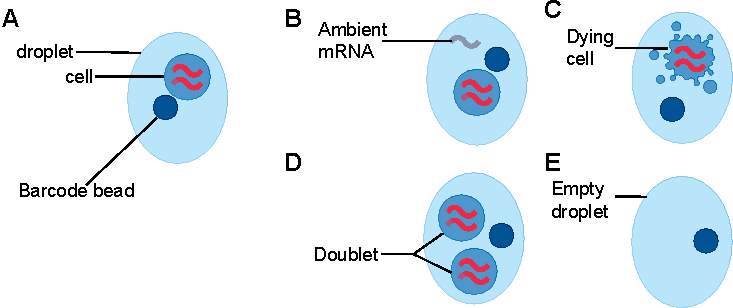
\includegraphics[width=0.95\textwidth]{PHLOWER_schematic/fig}
	\vspace{0.1cm}
	%\caption[Schematic overview of major steps of PHLOWER.]{xxxx}
	\caption[Schematic overview of major steps of PHLOWER.]{\textbf{Schematic overview of major steps of PHLOWER.} PHLOWER receives as input a multimodal or unimodal single cell data. \textbf{A)} It next creates a graph representation and a graph embedding (kamada-kawai algorithm) of the cells. Our example is based on a differentiation system of mouse embryonic fibroblasts (MEF) towards neurons or myocytes~\citep{treutlein2016dissecting}. From this graph, PHLOWER uses a zero order Laplacian decomposition and random-walk to estimate pseudo-time from progenitor cells (i.e. MEF). \textbf{B)}, Next, a simplicial complex (SC) is obtained by Delaunay triangulation of the graph represented in the kamada-kawai embedding and connecting cells end state cells with progenitor cells \textbf{C)} An edge embedding is obtained via the decomposition of the Hodge-Laplacian. In the MEF data, the first two eigenvectors have zero eigen-vectors and their signals discriminate edges belonging to the two differentiation trajectories (or holes in the SC). \textbf{D)} PHLOWER performs next random walks to obtain trajectories and uses the HL decomposition to obtain a trajectory embedding and a cumulative trajectory embedding. Clustering analysis in the trajectory embedding reveals major trajectories in the data, while the cumulative embedding space is used to estimate trajectory backbones and branching points events. PHLOWER outputs stream trees representing the differentiation tree over pseudo-time and allow the detection of regulators and gene markers.}
	\label{fig:PHLOWER_schematic}
\end{figure}

% python package dependencies
\begin{table}[!ht]
	\centering
	\begin{tabular}{lll}
		\toprule
		\textbf{Package} & \textbf{Version} & \textbf{Website} \\
		\midrule
			Numpy& >=1.23.5 & \url{https://numpy.org/} \\
			Matplotlib& >=3.6.0 & \url{https://matplotlib.org/} \\
			Seaborn& >=0.12.0 & \url{https://seaborn.pydata.org/} \\
			Pydot& >=1.4.2 & \url{https://github.com/pydot/pydot} \\
			Igraph& >=0.10.5 & \url{https://igraph.org/python/} \\
			Scikit-learn& >=1.1.2 & \url{https://scikit-learn.org/stable/} \\
			Scipy& >=1.10.1 & \url{https://www.scipy.org/} \\
			Pandas& >=1.3.5 & \url{https://pandas.pydata.org/} \\
			Plotly& >=5.13.1 & \url{https://plotly.com/} \\
			Tqdm& >=4.64.1 & \url{https://github.com/tqdm/tqdm} \\
			Leidenalg& >=0.9.1 & \url{https://github.com/vtraag/leidenalg} \\
			%louvain& >=0.8.0 & \url{} \\
			Colorcet& >=3.0.1 & \url{https://github.com/holoviz/colorcet} \\
			Umap-learn& >=0.5.3 & \url{https://github.com/lmcinnes/umap} \\
			Scikit-sparse& >=0.4.8 & \url{https://github.com/scikit-sparse/scikit-sparse} \\
			Scanpy& >=1.9.3 & \url{https://github.com/scverse/scanpy} \\
			Anndata& >=0.8.0 & \url{https://github.com/scverse/anndata} \\
            Magic-impute & >=0.8.03.0.0 & \url{https://github.com/KrishnaswamyLab/MAGIC}\\
		\bottomrule
	\end{tabular}
	\vspace{0.1cm}
	\caption[PHLOWER tool python package dependencies]{PHLOWER tool python package dependencies.}
	\label{tab:phlower_python_dependencies}
\end{table}
% a table shows the python dependencies
% check how to rotate the title text of a table, see Li's table 3.2

\section{Implementation}
\label{TI_methods:implementation}
We developed our Graph Hodge Laplacian (HL)-based approach to address the trajectory inference (TI) of single-cell multimodal data as a Python module. Our method is named PHLOWER (\textit{decom}\textbf{P}osition of the \textbf{H}odge \textbf{L}aplacian for inferring traject\textbf{O}ries from flo\textbf{W}s of c\textbf{E}ll diffe\textbf{R}entiation) and will be referred to as such throughout this thesis. The method's implementation encompasses all the steps described in this chapter. PHLOWER was initially released in September 2023. \fref{fig:PHLOWER_schematic} illustrates the workflow of PHLOWER, and \tref{tab:phlower_python_dependencies} summarizes the dependencies of the PHLOWER module.

PHLOWER requires, at a minimum, dimensional reduction as input as well as a count matrix to be processed by itself. The output of PHLOWER is a STREAM tree as visualization that shows the cell differentiation tree. In addition, PHLOWER outputs a tree structure with detailed random walk paths for downstream analysis.

By default, PHLOWER is designed to work seamlessly with Scanpy and Episcanpy. It also offers a range of analysis methods for cell differentiation downstream. For example, `phlower.tl.tree\_mbranch\_markers' is used to find significant markers for each branch against the rest of the branches. Moreover, for multimodal data, such as single-cell transcriptome and open chromatin, one can call `phlower.tl.branch\_TF\_gene\_correlation' to correlate two features along tree branches. With this, one can create a heatmap matrix using the function `phlower.tl.branch\_heatmap\_matrix' to show the features along the trajectories.

To ensure users utilize PHLOWER correctly, we have deployed PHLOWER documents to \url{https://phlower.readthedocs.io/en/latest/}, where one can easily check the vignette for using PHLOWER, as well as the API.

We have tested PHLOWER with Python (3.8-3.10) and required dependencies, such as Numpy 1.23.5, Matplotlib 3.8.1, Seaborn 0.13.0, Pydot 1.4.2, Igraph 0.10.5, Scikit-learn 1.1.2, Scipy 1.10.1, Pandas 2.0.3, Plotly 5.13.1, Tqdm 4.64.1, Leidenalg 0.9.1, Louvain 0.8.0, Colorcet 3.0.1, Umap-learn 0.5.3, Scikit-sparse 0.4.8, Episcanpy 0.4.0, Scanpy 1.9.3, Anndata 0.9.2, Magic-impute 3.0.0.

We executed PHLOWER on a local Linux Mint 21.1 x86\_64 64-bit machine with 12 Intel(R) Core(TM) i5-10400 CPUs at 2.90GHz and 64 GB RAM. Additionally, we ran PHLOWER on a High-Performance Computing (HPC) cluster primarily based on AMD EPYC 7452 64-bit nodes at 2.35 GHz and 500 GB RAM with Rocky Linux 8.9.

For more information about PHLOWER implementation, source code, tutorials and examples, please see:
\begin{center}
\url{https://github.com/CostaLab/phlower}
\end{center}

\section{Statistical Methods}
xxx
\section{Discussion}
\label{TI_methods:discussion}
In this chapter, we discussed our computational methods for single-cell multimodal trajectory inference. We first introduce, next xxx
Finally, we described the implementation details(sref{})

From a conceptual standpoint, when comparing our method of Hodge Laplacian decomposition with competing methods, it becomes evident that the latter either connect clusters to derive trajectories or identify backbones in low dimensions (2,3) to represent trajectories. However, none of these methods effectively utilizes the high dimensions of a graph for inference. In contrast, our method utilizes edges in the high-dimensional cumulative trajectory space to identify branching points. This marks the first time Hodge Laplacian decomposition is employed to create a tree structure. Such innovation can find applications not only in biology but also in areas such as traffic detection and beyond.

\begin{itemize}

    \item We emphasized the utilization of high-level graph information, specifically the Hodge Laplacian, to capture not only relations between vertices and edges but also relations between edges and triangles. Leveraging more information allows us to derive more accurate trajectories for single-cell analysis.

    \item Subsequently, we developed a trajectory inference method based on the decomposition of the Hodge Laplacian. Our approach goes beyond a simple application of this theory to the single-cell trajectory inference problem. Incorporating essential elements such as hole creation and triangulation tricks, we address the nuances of the problem. Additionally, to overcome the issue of preference random walk getting stuck in local areas, we propose a two-step process. First, we perform the walk on the diffusion graph, followed by finding the shortest paths on the triangulated graph. The creation of a tree structure is also crucial, and we achieve this by calculating normalized distances for edges in the cumulative trajectory space to determine branching points

\end{itemize}


